\documentclass[UTF8,a4paper,12pt]{ctexart}

\usepackage[
  a4paper,
  top=2.5cm,
  bottom=2.5cm,
  left=2.5cm,
  right=2.5cm,
  headheight=16pt
]{geometry}
\usepackage{amsmath,amssymb,amsthm}
\usepackage{booktabs,longtable,array,multirow}
\usepackage{graphicx}
\usepackage{pdfpages}
\usepackage{tikz}
\usepackage{caption}
\usepackage{subcaption}
\usepackage{float}
\usepackage{enumitem}
\usepackage{setspace}
\usepackage{fancyhdr}
\usepackage{titlesec}
\usepackage{hyperref}
\usepackage{xcolor}
\usepackage{url}

\hypersetup{
  colorlinks=true,
  linkcolor=black,
  urlcolor=blue,
  citecolor=black,
  pdfauthor={RosiePenguin Team},
  pdftitle={“浙超”分组方案、抽签机制、赛点选择与赛制优化的一体化研究}
}

\setlength{\parindent}{2em}
\setlength{\parskip}{0.3em}
\onehalfspacing
\graphicspath{{../results/problem2/}{../results/problem34/}}
\captionsetup{font=small,labelsep=space}
\setlist[itemize]{leftmargin=2.5em}
\setlist[enumerate]{leftmargin=2.8em}

\pagestyle{fancy}
\fancyhf{}
\fancyhead[C]{“浙超”分组方案、抽签机制、赛点选择与赛制优化的一体化研究}
\fancyfoot[C]{\thepage}
\renewcommand{\headrulewidth}{0.4pt}
\renewcommand{\footrulewidth}{0pt}

\titleformat{\section}{\zihao{4}\bfseries}{\thesection}{0.75em}{}
\titleformat{\subsection}{\zihao{-4}\bfseries}{\thesubsection}{0.75em}{}
\titleformat{\subsubsection}{\zihao{5}\bfseries}{\thesubsubsection}{0.75em}{}

\begin{document}

\thispagestyle{empty}
\begin{center}
{\zihao{1}\bfseries 浙江大学第二十四届\par}
\vspace{0.2cm}
{\zihao{1}\bfseries 大学生数学建模竞赛\par}
\vspace{0.9cm}
{\zihao{3}2026年5月8日－5月18日\par}
\end{center}

\vspace{1.0cm}
\noindent
\hspace*{2.0cm}{\zihao{2}团队编号\ \underline{\makebox[3.0cm][c]{46}}}\par
\vspace{0.25cm}
\noindent
\hspace*{2.0cm}{\zihao{2}题\quad 目\qquad A \qquad B$\checkmark$}\par
\noindent
\hspace*{1.8cm}{\zihao{-3}（在所选题目上打勾）}\par

\vspace{0.35cm}
\renewcommand{\arraystretch}{1.55}
\begin{center}
\begin{tabular}{|>{\centering\arraybackslash}m{1.9cm}|>{\centering\arraybackslash}m{4.6cm}|>{\centering\arraybackslash}m{4.6cm}|>{\centering\arraybackslash}m{4.6cm}|}
\hline
 & 参赛队员1 & 参赛队员2 & 参赛队员3 \\
\hline
姓名 & 张若希 & 万里行 & 全炳旭 \\
\hline
学号 & 3240105081 & 3240105071 & 3240105082 \\
\hline
院（系） & 竺可桢学院 & 计算机科学与技术学院 & 竺可桢学院 \\
\hline
专业 & 图灵班（计算机科学与技术） & 人工智能 & 图灵班（计算机科学与技术） \\
\hline
手机 & 19706868927 &  & 15972240160 \\
\hline
Email & 3240105081@zju.edu.cn &  & quanbx@zju.edu.cn \\
\hline
\end{tabular}
\end{center}

\vspace{0.8cm}
\begin{center}
{\zihao{2}\bfseries 浙江大学本科生院\par}
\vspace{0.15cm}
{\zihao{2}\bfseries 浙江大学数学建模实践基地\par}
\end{center}
\clearpage

\pagenumbering{gobble}
\thispagestyle{empty}
\begin{center}
{\zihao{3}\bfseries 摘要}
\end{center}

针对“浙超”联赛 64 支队伍的小组分组、抽签公平性、比赛地点选择及赛制优化问题，本文构建了一套“分组生成—公平抽签—赛点配置—赛制优化”的一体化建模框架，将题目四问联结为一条可复现、可解释、可扩展的决策链。对于问题 1，本文将题目要求拆分为“市级队分散、直属回避、同市县级队尽量分散”三类约束，建立带硬约束与软约束的组合优化模型，并设计“市级队随机落位 + 县级队按约束紧度逐步安置”的随机启发式算法，在 500 次搜索中获得 450 个可行方案。最优方案实现了同市县级队同组冲突对数为 0、平均城市来源熵为 2.0000、各组总实力标准差为 6.2099，表明该方案在公平性、分散性与竞技均衡性之间达到了较好平衡。对于问题 2，本文设计分阶段等概率抽签流程，并通过 10000 次蒙特卡洛模拟和卡方检验验证其公平性。结果显示，64 支队伍的平均 $p$ 值为 0.5418，无队伍出现 $p < 0.01$ 的显著偏差，仅有 4 支队伍满足 $p < 0.05$，与纯随机条件下的正常波动一致，因此抽签方案在统计意义上公平、透明且具有可实施性。对于问题 3，本文基于浙江省 64 个参赛地区的人口、GDP、交通、体育基础、铁路与机场可达性、代表性场馆容量等数据，构建熵权多目标离散设施选址模型，将“平均旅行距离、最远旅行距离、公平性、赛事影响力、承办能力”统一纳入综合效用函数，最终推荐三门县、诸暨市、仙居县、丽水市、义乌市、东阳市、磐安县和金华市 8 个赛点，平均分配距离为 127.83\,km，最大距离为 214.82\,km，且无主场惩罚触发，说明所给赛点方案同时兼顾了参赛便利、公平分布与赛事传播效应。对于问题 4，本文根据地区综合指标构建队伍实力代理值，并引入基于旅行负担的疲劳项，搭建包含小组赛、淘汰赛、加时赛与点球大战的比赛仿真模型，对 7 类候选赛制进行了 20000 次蒙特卡洛比较。结果表明，\texttt{seeded\_reseeded} 方案在优先级加权 TOPSIS 下得分最高，为 0.822888；与当前随机赛制相比，该方案将前 4 强队在 32 强首轮出局概率由 0.2831 降至 0.2551，将前 8 强队进入八强的概率由 0.3817 提高到 0.3968，说明“32 强种子保护 + 16 强后复排”能够更有效减少强队过早相遇。进一步地，本文从约束处理、指标体系、疲劳建模和敏感性分析四个方面提出模型改进：将问题 1 从单一可行性搜索提升为多方案比较；将问题 3 从单纯地理邻近扩展为多目标离散选址；将问题 4 从静态对阵比较提升为带旅行疲劳的动态仿真；并对权重与参数变化进行了稳健性检验。研究表明，本文方法不仅能够解决本题，还可推广到区域足球联赛、校际联赛和其他多赛点淘汰类赛事的赛务组织决策。

\vspace{0.8em}
\noindent\textbf{关键词：}分组优化；公平抽签；设施选址；蒙特卡洛模拟；熵权法；TOPSIS

\clearpage
\pagenumbering{arabic}

\section{问题重述}

“浙超”联赛共有 64 支队伍参赛，其中包括 11 支市级队、20 支县级市队和 33 支县队。比赛分为两个阶段：第一阶段为 16 个小组、每组 4 队的单循环小组赛，小组前两名晋级；第二阶段为 32 强淘汰赛，经过 5 轮决出冠军。题目要求分别解决以下四个问题：

\begin{enumerate}
  \item 在满足行政回避和分散原则的前提下给出若干可行分组方案，并比较其优劣。
  \item 设计公平、透明且可实施的抽签流程，并验证其公平性。
  \item 根据分组结果选择 8 个比赛地点，每个赛点承办 2 个小组，兼顾公平、便利和赛事影响力。
  \item 结合足球比赛特征，利用数学模型与定量分析对赛制提出改进建议。
\end{enumerate}

这四个问题具有明显的前后依赖关系：问题 1 的分组结果决定问题 2 的合法抽签空间，也为问题 3 的赛点选择提供输入；问题 3 的出行负担又会影响问题 4 的疲劳与赛制评价。因此，本文不将四问割裂处理，而是构建统一的一体化建模框架。

\section{问题分析}

问题 1 本质上是一个大规模带约束分配问题。若直接枚举 64 支队伍分入 16 个小组的所有方案，其组合规模极为庞大，不可能通过穷举获得结果。因此需要构造能快速生成可行解并支持多方案比较的启发式算法。

问题 2 的难点并不在于“抽出一个合法分组”，而在于要证明抽签规则对所有队伍没有系统性偏置，即长期运行下的边际分配概率应接近均匀。因此仅给出抽签流程还不够，还必须给出统计公平性的定量证据。

问题 3 并不是简单挑选“最强城市”或“最近城市”，而是一个同时受小组配对、赛点唯一性、出行公平、赛事影响和承办能力共同约束的多目标离散设施选址问题。若只关注某一个目标，例如总距离最小，往往会牺牲赛事传播面或承办质量。

问题 4 需要比较多种赛制对“强队保护”“比赛公平”“旅行负担”和“筛选效率”的影响。由于比赛结果具有随机性，适合用蒙特卡洛仿真进行大样本统计比较，而不宜采用简单经验判断。

\section{模型假设}

为保证模型可计算且结论可解释，本文作如下假设：

\begin{enumerate}
  \item 64 支队伍全部按题意参赛，不考虑中途退赛或资格变更。
  \item 行政隶属关系固定，市级队与其代管县级队的回避关系不发生变化。
  \item 在缺乏完整历史战绩时，使用地区综合指标构造球队实力代理值。
  \item 抽签设备与程序在技术上等概率执行，不存在人为操控。
  \item 比赛出行成本主要由地理距离和交通可达性刻画。
  \item 比赛结果由实力差、疲劳与随机扰动共同决定，不单独建模天气、伤病与裁判因素。
\end{enumerate}

\section{符号说明}

\begin{table}[H]
\centering
\caption{主要符号说明}
\begin{tabular}{>{\centering\arraybackslash}p{0.16\textwidth} p{0.7\textwidth}}
\toprule
符号 & 含义 \\
\midrule
$G$ & 小组集合，$|G|=16$ \\
$T$ & 参赛队伍集合，$|T|=64$ \\
$C$ & 市级队集合，$|C|=11$ \\
$x_{ig}$ & 队伍 $i$ 是否分入小组 $g$ 的 0-1 变量 \\
$P$ & 同市县级队在同组形成的冲突对数 \\
$H$ & 各组来源城市熵的平均值 \\
$\sigma_s$ & 各组总实力标准差 \\
$S_{pv}$ & 小组对 $p$ 分配到赛点 $v$ 时的综合得分 \\
$I_v$ & 赛点 $v$ 的赛事影响指标 \\
$K_v$ & 赛点 $v$ 的承办能力指标 \\
$F_m$ & 赛制方案 $m$ 的综合评价得分 \\
\bottomrule
\end{tabular}
\end{table}

\section{问题 1：分组方案生成与评价模型}

\subsection{约束建模}

本文将题目中的分组条件拆分为三类：

\begin{enumerate}
  \item 每支队伍恰分入一个小组，每组恰有 4 支队伍；
  \item 11 支市级队必须位于 11 个不同小组；
  \item 若某组已有某市市级队，则该市代管县级队不得进入该组。
\end{enumerate}

其中前三条属于硬约束；“同一市代管县级队尽量不分在同组”属于软约束。为量化软约束，定义同市县级队在同组形成的冲突对数
\[
P=\sum_{g\in G}\sum_c \binom{n_{gc}}{2},
\]
其中 $n_{gc}$ 为小组 $g$ 中来自城市 $c$ 的县级队数。显然，$P$ 越小越好。

\subsection{随机启发式算法}

考虑到组合规模过大，本文采用两阶段随机启发式算法：

\begin{enumerate}
  \item 先随机为 11 支市级队分配 11 个互不相同的小组位置；
  \item 再按“约束更紧者优先”的原则逐一放置县级队；
  \item 对于每支县级队，优先在不与同源县级队冲突、且组内人数较少的合法小组中随机选取；
  \item 多次独立搜索后保留全部可行方案，并按综合指标排序。
\end{enumerate}

\subsection{评价指标与综合得分}

本文用以下三个指标评价分组方案：

\begin{itemize}
  \item \texttt{soft\_conflict\_pairs}：同市县级队同组冲突对数，越小越好；
  \item \texttt{avg\_city\_entropy}：各组来源城市熵的平均值，越大越好；
  \item \texttt{strength\_balance\_std}：各组总实力标准差，越小越好。
\end{itemize}

综合得分设为
\[
Score = 100H - 15P - 2\sigma_s.
\]
该表达式兼顾分散性、公平性与竞技均衡性。

\subsection{结果分析}

程序共搜索 500 次，得到 450 个可行方案，最优方案结果如表 \ref{tab:problem1} 所示。

\begin{table}[H]
\centering
\caption{问题 1 最优分组方案指标}
\label{tab:problem1}
\begin{tabular}{lc}
\toprule
指标 & 数值 \\
\midrule
可行方案数 & 450 \\
同市县级队同组冲突对数 & 0.0 \\
平均城市熵 & 2.0000 \\
各组总实力标准差 & 6.2099 \\
综合得分 & 187.5803 \\
\bottomrule
\end{tabular}
\end{table}

该结果说明：第一，全部硬约束均被满足；第二，软约束冲突完全消除；第三，小组整体实力保持较高均衡度。因此，问题 1 不仅给出了一个“合法方案”，还给出了一个可比较、可解释的优选方案。

\section{问题 2：公平抽签方案设计与验证}

\subsection{抽签机制设计}

本文设计的抽签机制采用“市级队先抽、县级队后抽”的分阶段流程：

\begin{enumerate}
  \item 市级队随机进入 16 个小组中的 11 个不同小组；
  \item 县级队随后在实时更新的合法小组集合中进行等概率抽签；
  \item 若存在不与同市县级队相遇的严格合法集合，则优先在该集合内随机抽取。
\end{enumerate}

这一流程既满足题目约束，也便于在线下抽签中用“签池 + 回避规则”的方式直观实现。

\subsection{公平性检验}

本文进行了 10000 次蒙特卡洛模拟，并对每支队伍落入各组的频数分布进行卡方检验。统计结果如下：

\begin{itemize}
  \item 平均 $p$ 值：0.5418；
  \item $p < 0.01$ 的队伍数：0；
  \item $p < 0.05$ 的队伍数：4；
  \item 纯随机情况下理论期望 $p < 0.05$ 数：3.2。
\end{itemize}

上述结果表明，抽签偏差并未超出纯随机波动应有范围，因此可认为该抽签方案在统计意义上公平。

\begin{figure}[H]
\centering
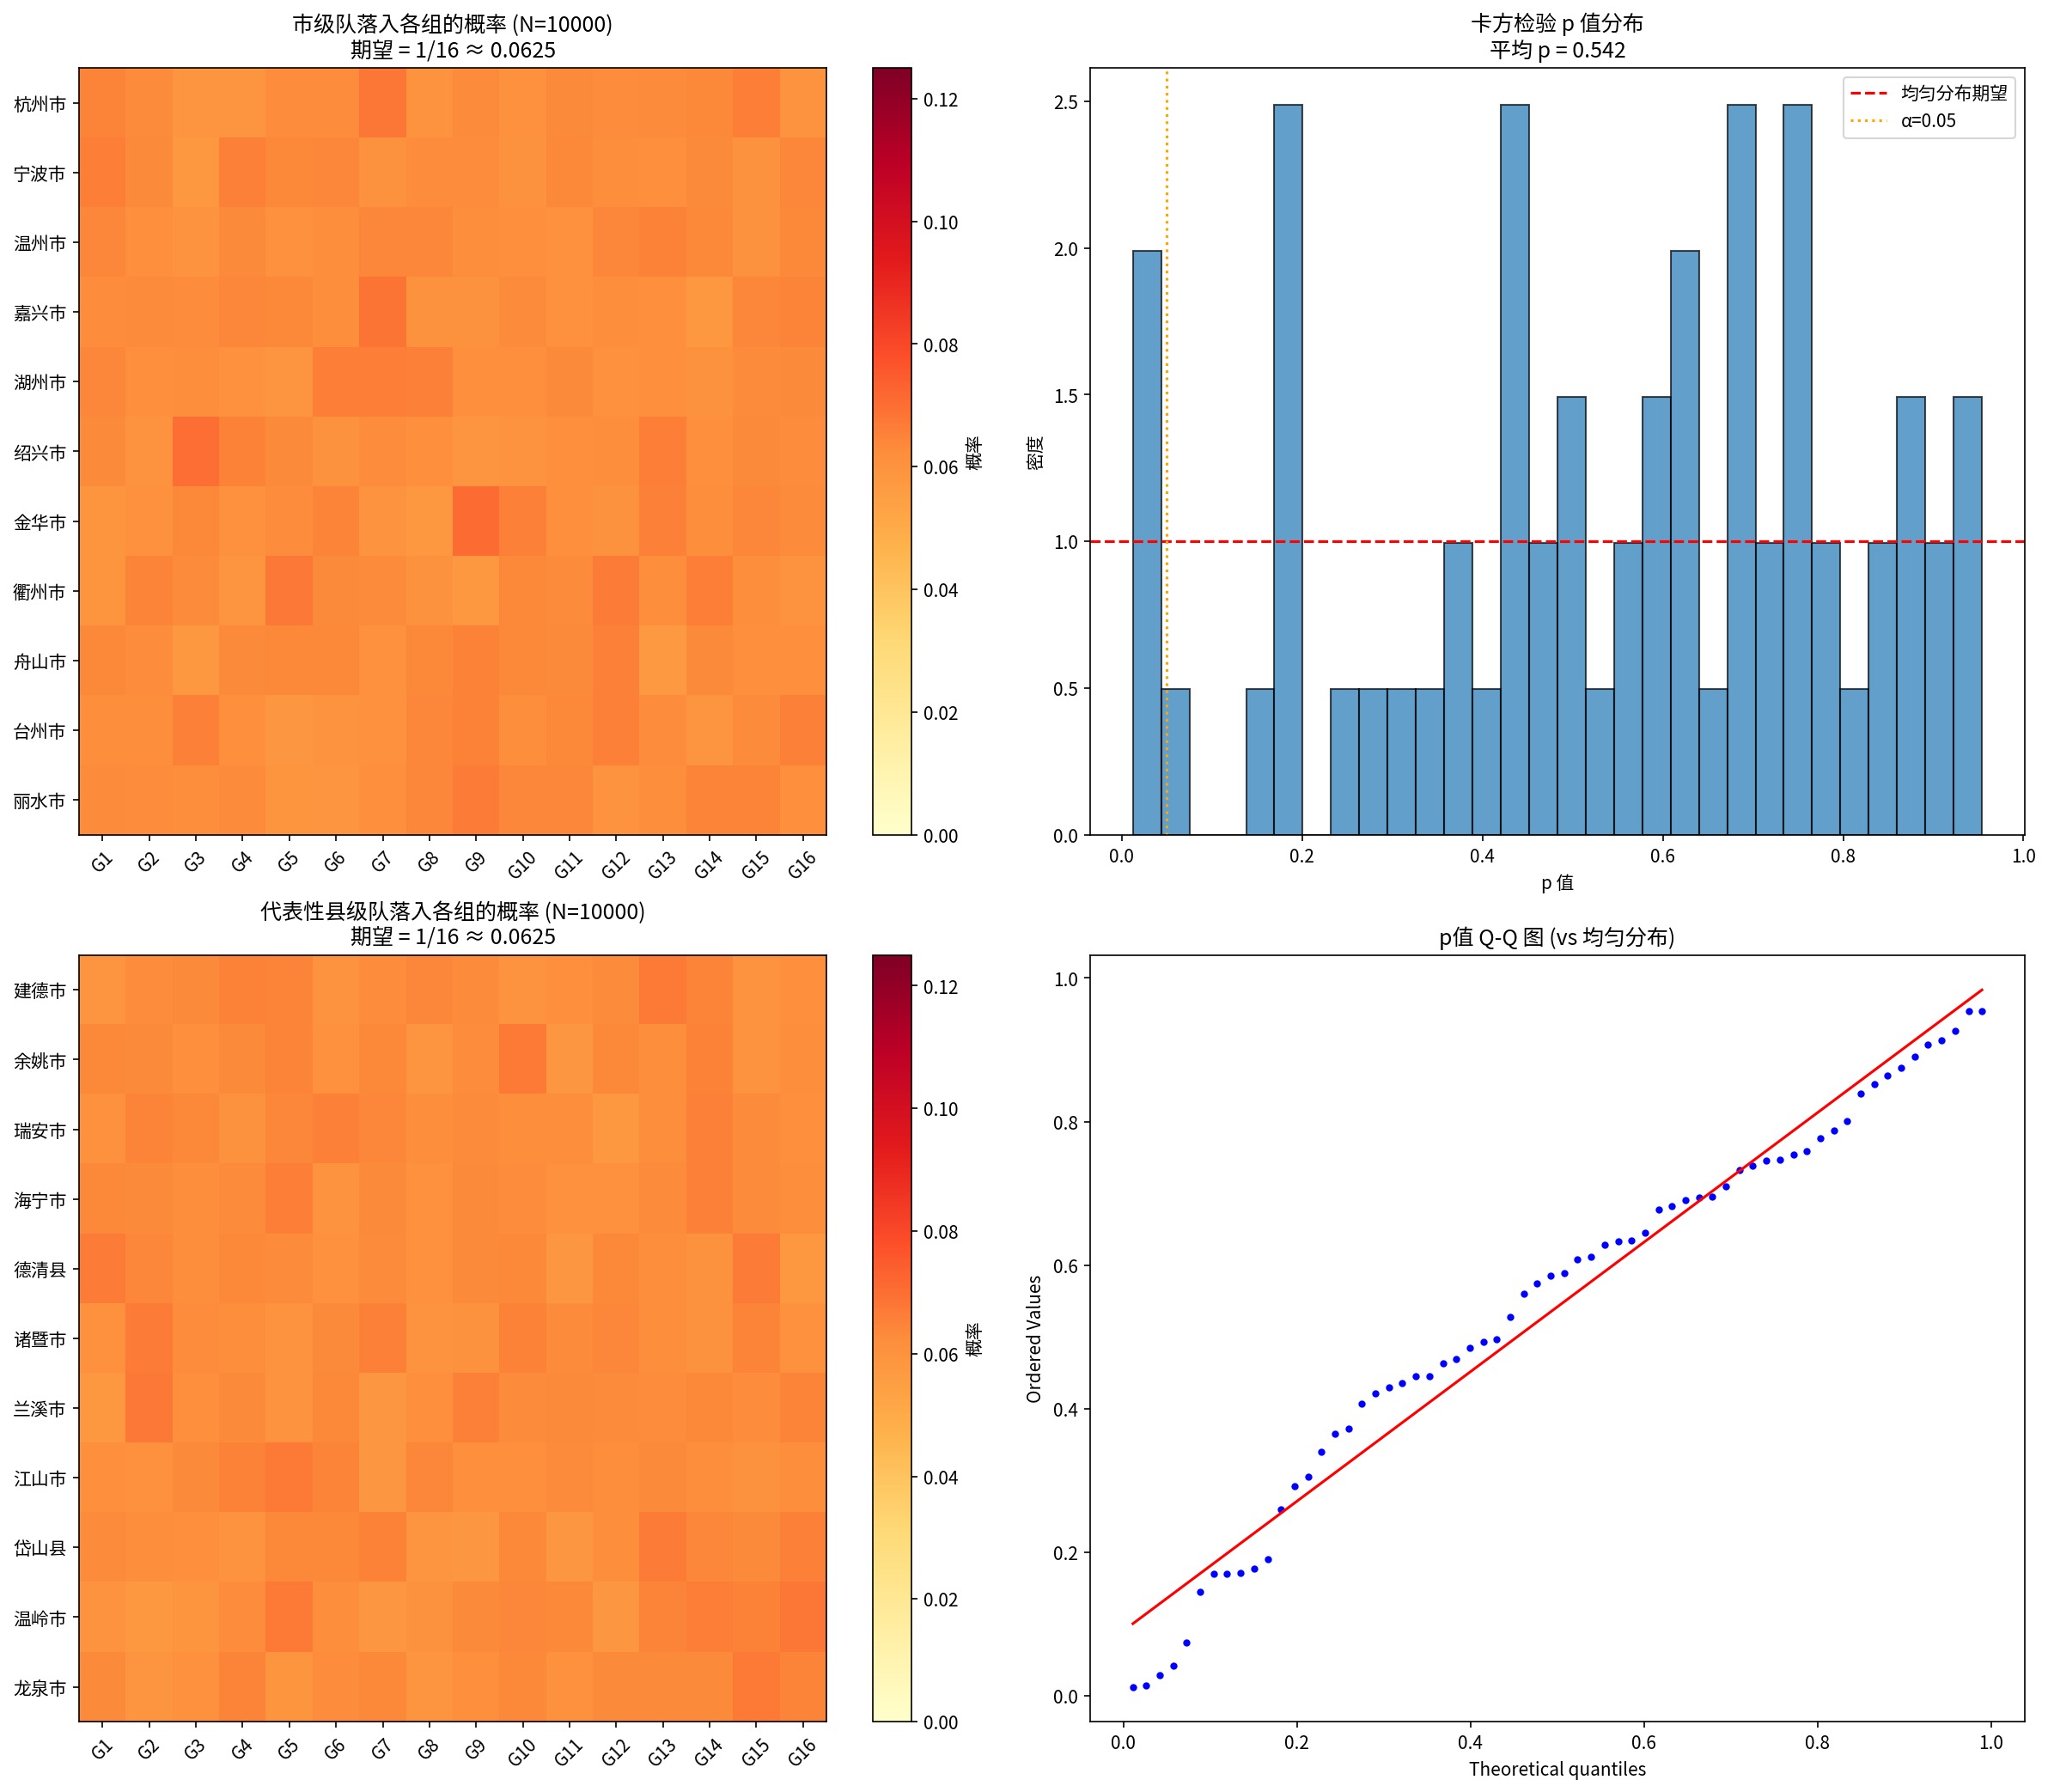
\includegraphics[width=0.9\textwidth]{fairness_analysis.png}
\caption{抽签公平性统计图}
\label{fig:fairness}
\end{figure}

图 \ref{fig:fairness} 展示了市级队和代表性县级队落入各组的概率热力图、$p$ 值分布与 Q-Q 图。整体上，各队落入 16 个小组的边际概率与理论值 $1/16$ 基本一致。

\begin{figure}[H]
\centering
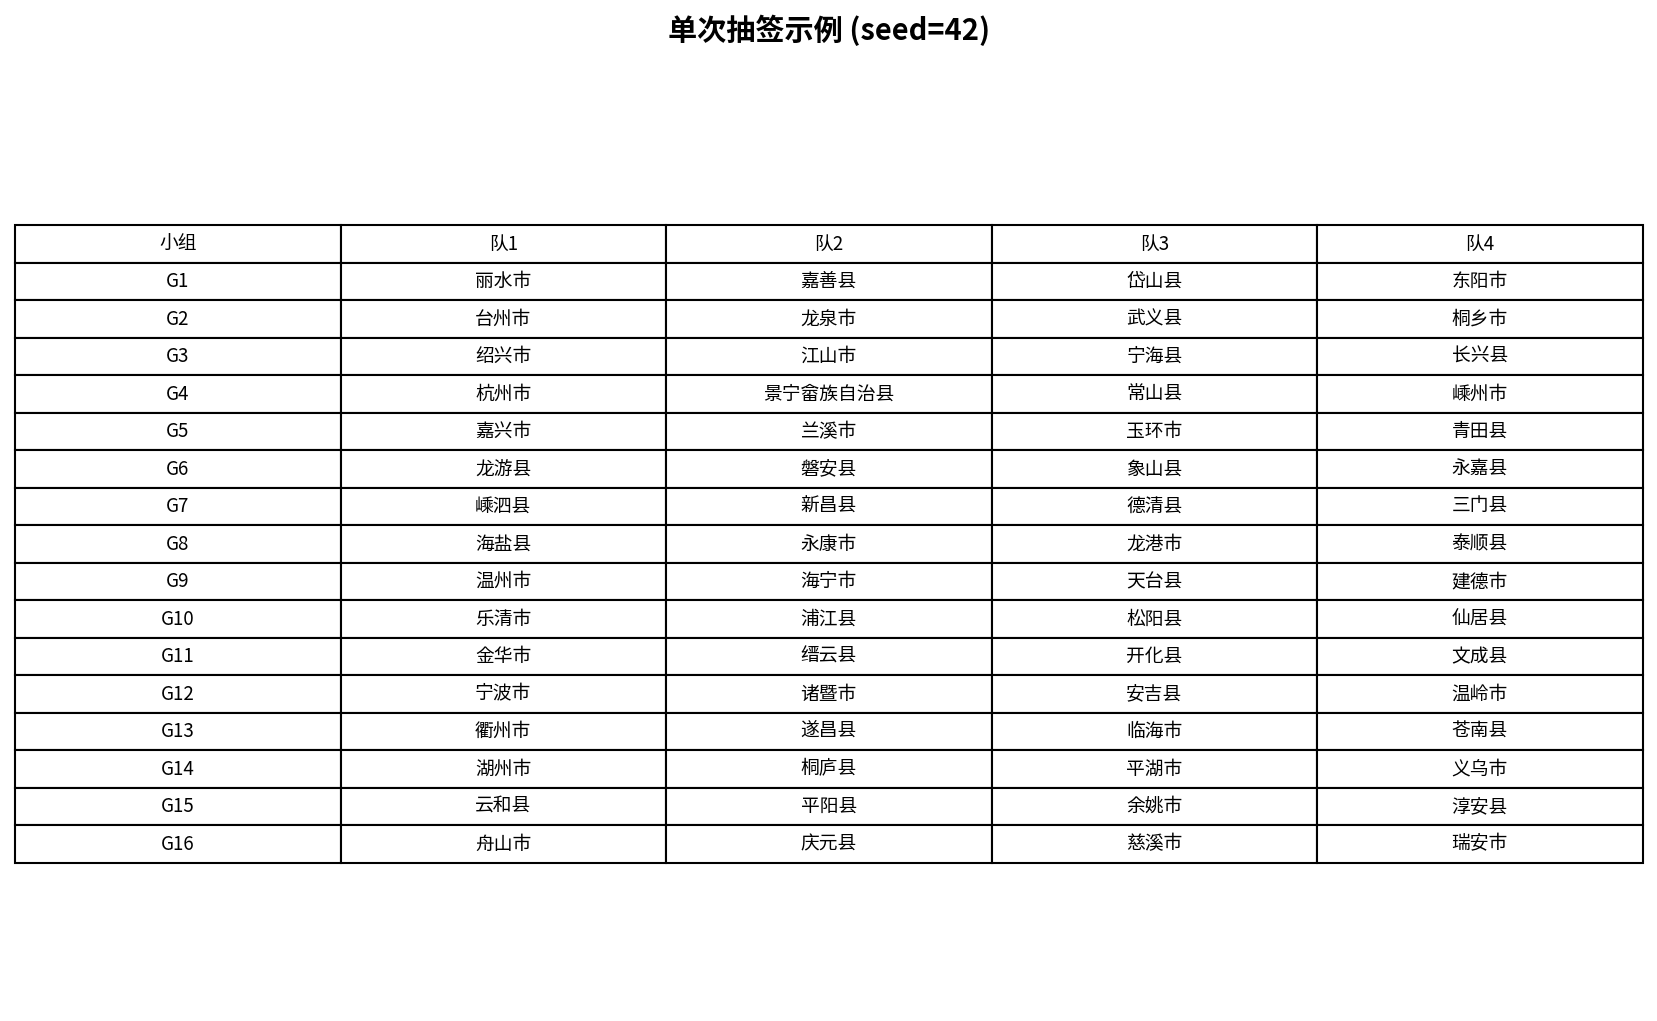
\includegraphics[width=0.82\textwidth]{draw_example.png}
\caption{单次抽签示例}
\label{fig:draw-example}
\end{figure}

图 \ref{fig:draw-example} 给出了一次代表性抽签结果，直观展示了“市级队分散 + 直属回避 + 县级队尽量分散”的综合效果。

\section{问题 3：比赛地点选择模型}

\subsection{数据体系构建}

本文利用 64 个参赛地区的人口、GDP、交通、体育基础、铁路可达性、机场可达性及代表性场馆容量等信息，建立了赛事影响力与承办能力双层指标体系。其中：

\begin{itemize}
  \item 赛事影响力由人口、GDP、交通和足球氛围构成；
  \item 承办能力由体育基础、场馆容量、铁路可达性和机场可达性构成。
\end{itemize}

各指标经归一化后采用熵权法确定权重。

\subsection{多目标离散设施选址模型}

设 16 个小组需两两配对后分配给 8 个赛点。对于任意小组对 $p$ 和候选赛点 $v$，定义综合效用函数
\[
S_{pv}=w_1A_{pv}+w_2W_{pv}+w_3F_{pv}+w_4I_v+w_5K_v-\mathrm{Penalty}_{pv},
\]
其中 $A_{pv}$ 为平均旅行便利度，$W_{pv}$ 为最远旅行控制项，$F_{pv}$ 为公平性得分，$I_v$ 为赛事影响力，$K_v$ 为承办能力，$\mathrm{Penalty}_{pv}$ 为主场惩罚项。

模型在满足“小组全部被覆盖、赛点不重复、每个赛点承办两个小组”的条件下，最大化 8 个小组对的综合效用之和。

\subsection{结果分析}

主方案推荐的 8 个赛点如表 \ref{tab:problem3} 所示。

\begin{table}[H]
\centering
\caption{问题 3 推荐赛点方案}
\label{tab:problem3}
\begin{tabular}{lccc}
\toprule
赛点 & 承办小组 & 平均距离/km & 最大距离/km \\
\midrule
三门县 & G01+G02 & 163.65 & 209.14 \\
诸暨市 & G03+G12 & 120.81 & 157.00 \\
仙居县 & G04+G09 & 94.14 & 145.57 \\
丽水市 & G05+G15 & 105.25 & 153.06 \\
义乌市 & G06+G14 & 136.61 & 176.51 \\
东阳市 & G07+G10 & 106.19 & 150.84 \\
磐安县 & G08+G11 & 162.17 & 214.82 \\
金华市 & G13+G16 & 133.80 & 181.39 \\
\bottomrule
\end{tabular}
\end{table}

整体结果表明：平均分配距离为 127.83\,km；最大分配距离为 214.82\,km；主场惩罚触发次数为 0。这说明推荐方案在控制极端出行负担的同时，没有通过明显主场便利来换取得分，因此具有较好的公平性与可实施性。

\begin{figure}[H]
\centering
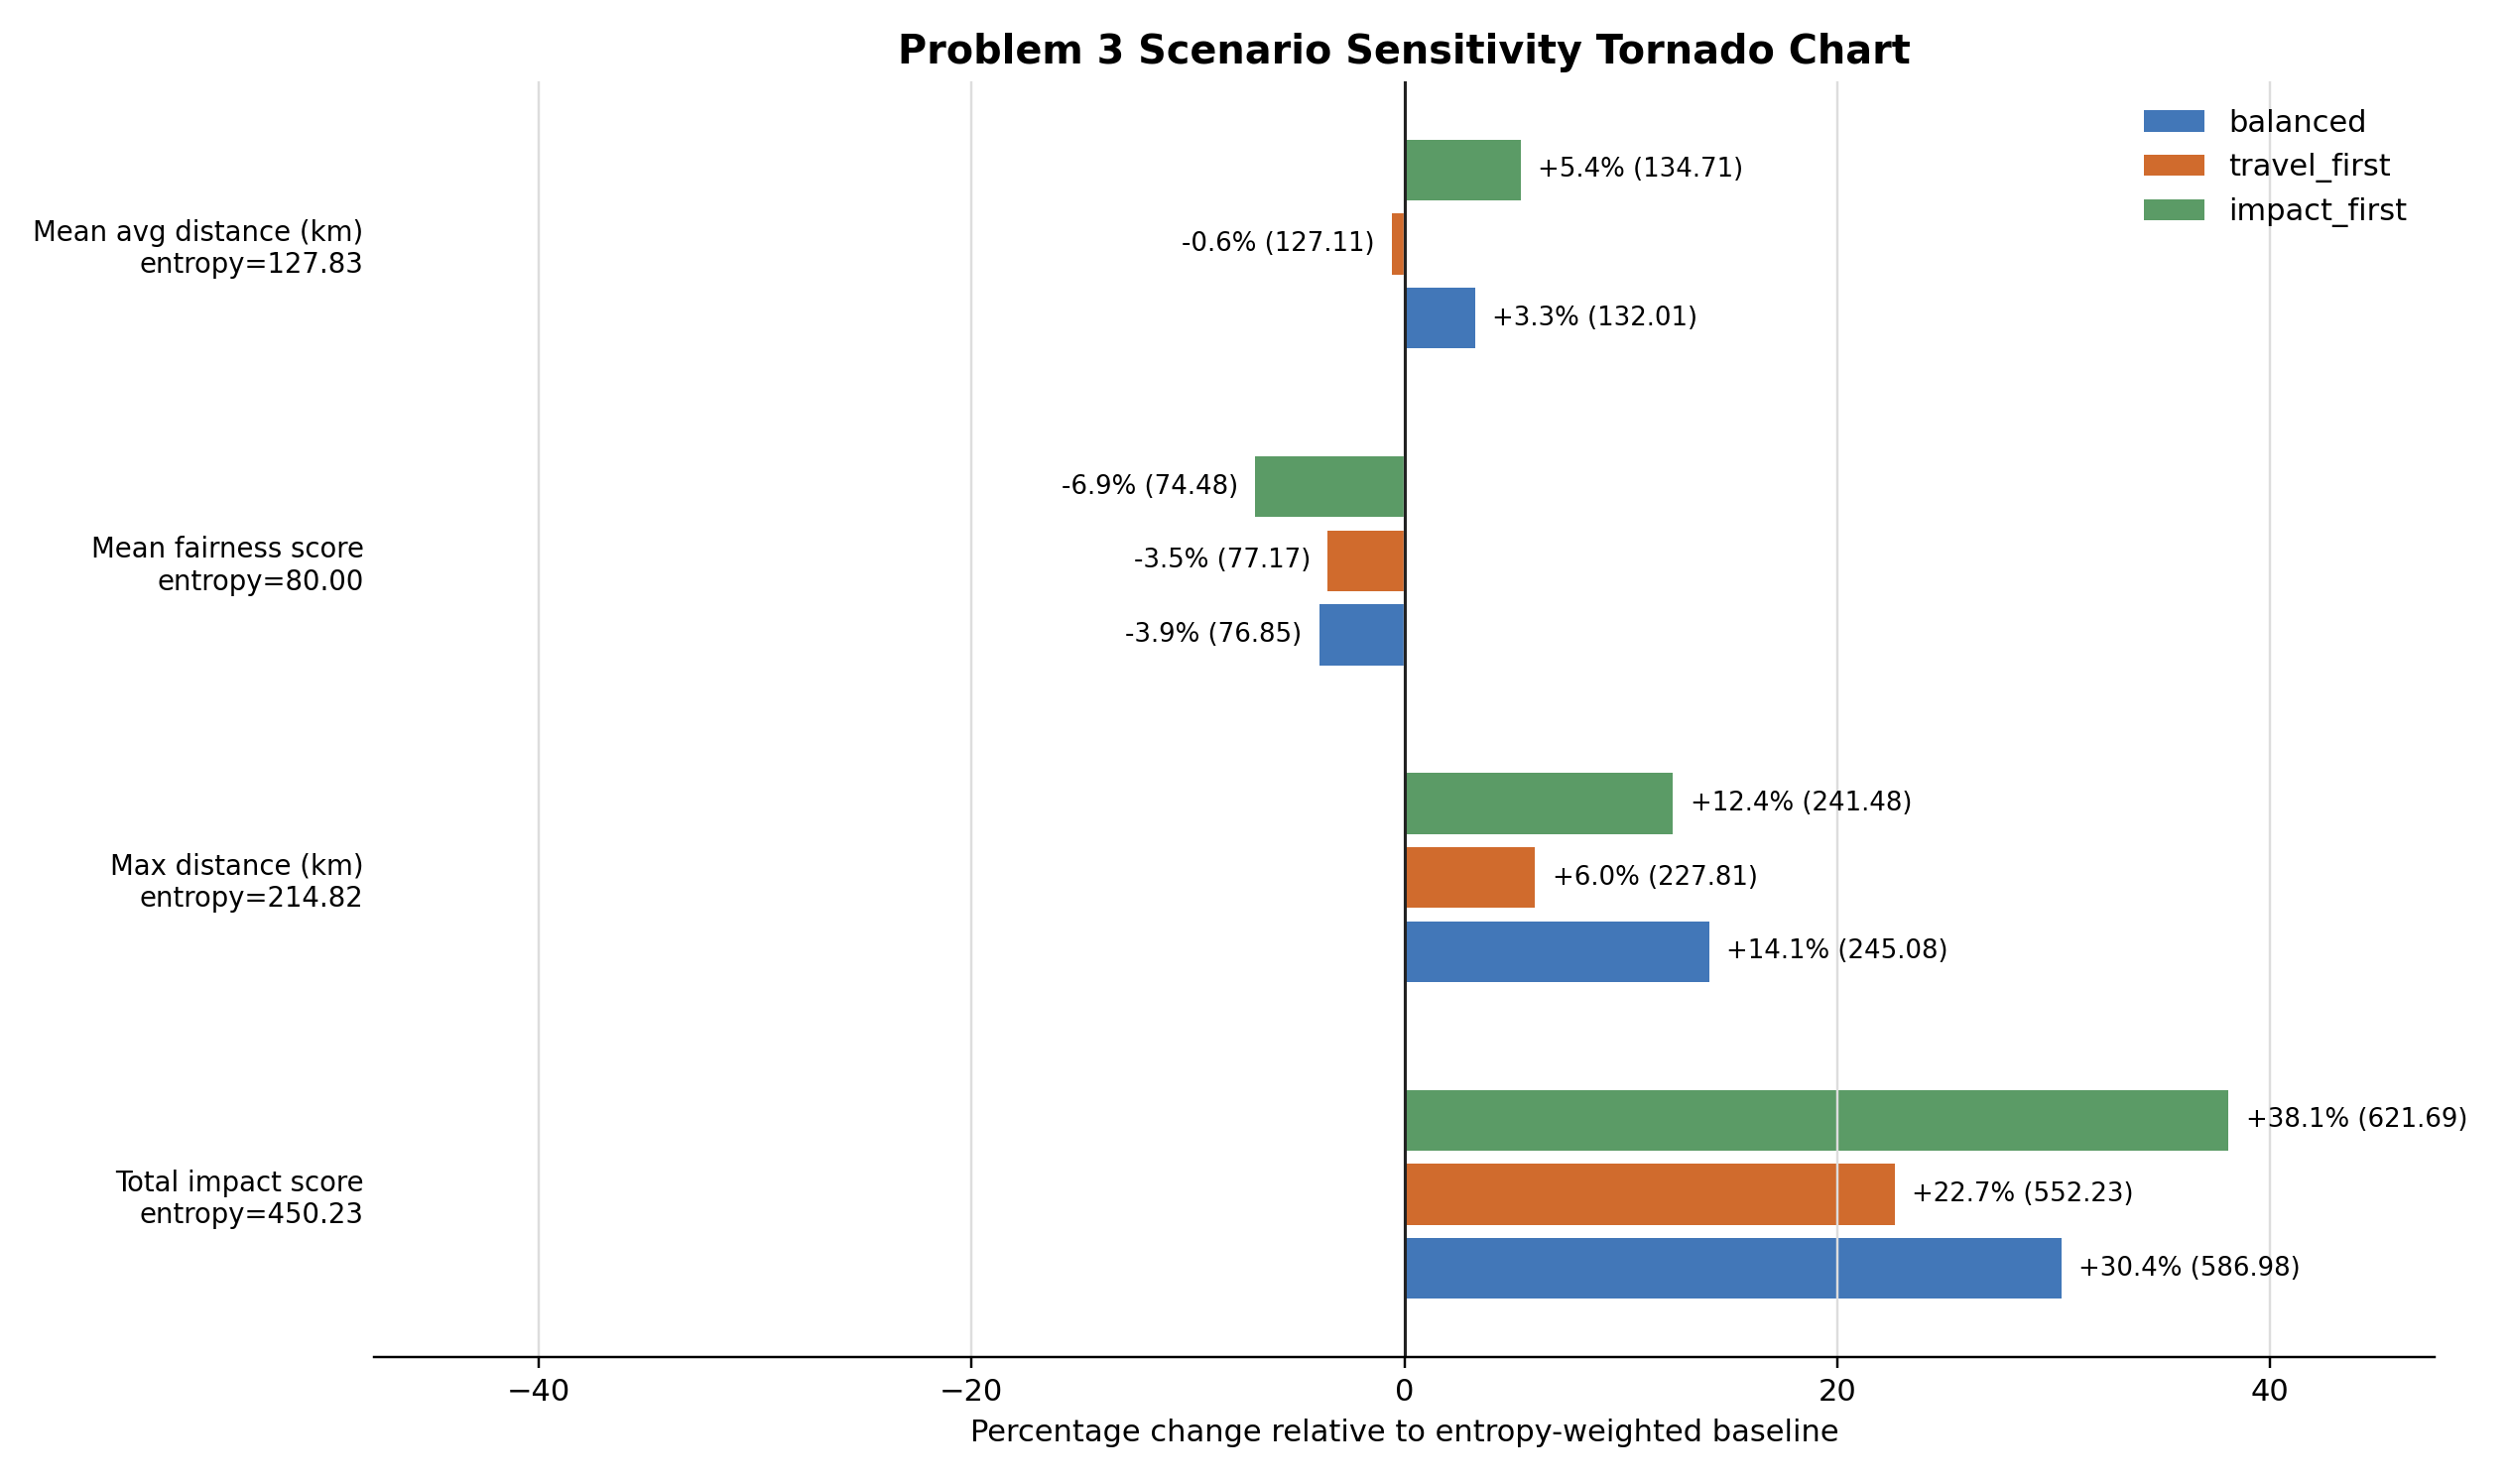
\includegraphics[width=0.78\textwidth]{problem3_typhoon_sensitivity.png}
\caption{赛点方案对极端天气权重的敏感性}
\label{fig:problem3-sensitivity}
\end{figure}

图 \ref{fig:problem3-sensitivity} 表明，在不同天气风险权重设定下，核心赛点组合总体稳定，说明选址模型具有一定稳健性。

\section{问题 4：赛制优化模型}

\subsection{实力代理与疲劳机制}

考虑到缺乏完整历史战绩，本文基于人口、GDP、交通、足球氛围和体育基础 5 项指标构造队伍实力代理值。随后引入基于旅行距离的疲劳项，将其嵌入比赛仿真模型中，从而更真实地反映赛点选择对后续淘汰赛的影响。

\subsection{候选赛制与评价指标}

本文比较以下 7 类赛制：

\begin{itemize}
  \item \texttt{current\_random\_draw}
  \item \texttt{random\_draw\_rest}
  \item \texttt{random\_draw\_reseeded}
  \item \texttt{group\_rank\_seeded}
  \item \texttt{group\_rank\_seeded\_rest}
  \item \texttt{seeded\_reseeded}
  \item \texttt{seeded\_reseeded\_rest}
\end{itemize}

评价指标为：

\begin{itemize}
  \item 冠军平均实力；
  \item 前 8 强队进入八强概率；
  \item 前 4 强队在 32 强首轮出局概率；
  \item 高出行负担队伍进入八强概率。
\end{itemize}

最终采用优先级加权 TOPSIS 进行综合排序。

\subsection{仿真结果}

关键结果如表 \ref{tab:problem4} 所示。

\begin{table}[H]
\centering
\caption{问题 4 候选赛制比较}
\label{tab:problem4}
\begin{tabular}{lccc}
\toprule
赛制 & 前 8 队进八强率 & 前 4 队首轮出局率 & TOPSIS \\
\midrule
\texttt{current\_random\_draw} & 0.3817 & 0.2831 & 0.258954 \\
\texttt{group\_rank\_seeded} & 0.3894 & 0.2575 & 0.662609 \\
\texttt{seeded\_reseeded} & 0.3968 & 0.2551 & 0.822888 \\
\texttt{seeded\_reseeded\_rest} & 0.3931 & 0.2591 & 0.706284 \\
\bottomrule
\end{tabular}
\end{table}

结果表明，\texttt{seeded\_reseeded} 方案在综合评价中最优。它一方面能够提高强队进入后续轮次的概率，另一方面又能降低强队在 32 强阶段过早相遇的风险。

\begin{figure}[H]
\centering
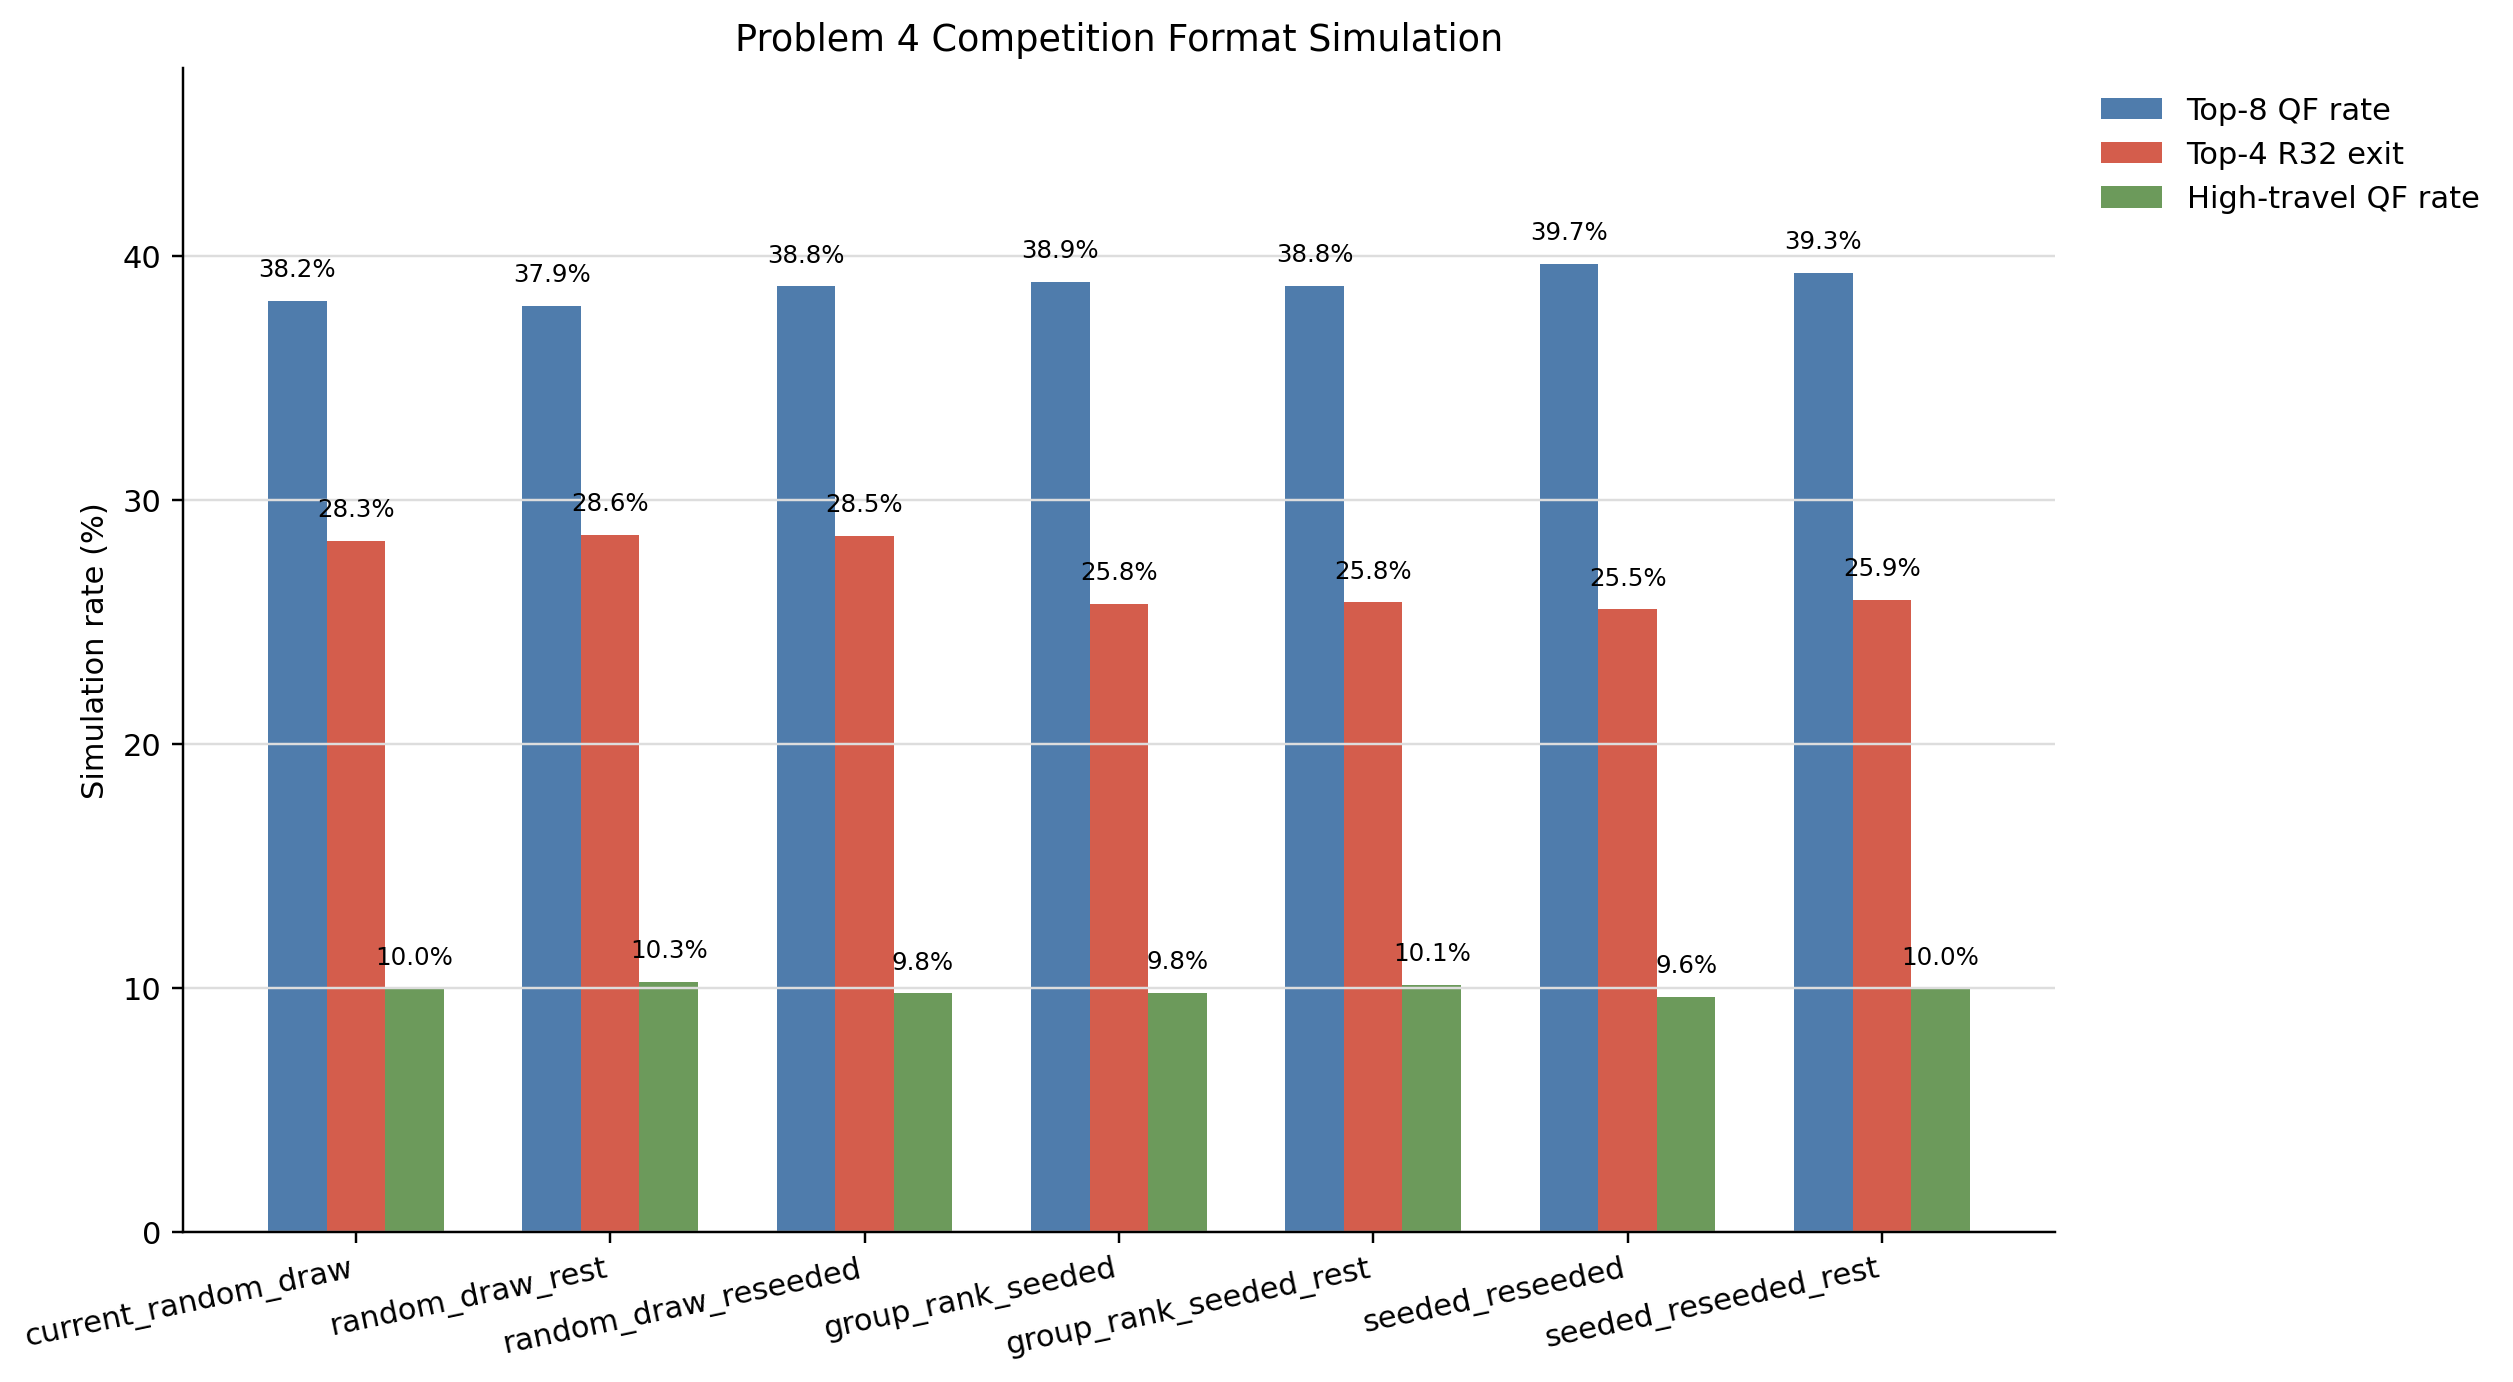
\includegraphics[width=0.82\textwidth]{problem4_format_comparison.png}
\caption{各候选赛制的综合比较}
\label{fig:problem4-comparison}
\end{figure}

因此，本文建议保留现有小组赛结构，在 32 强阶段采用“小组第一对小组第二”的种子保护方式，并在 16 强以后依据小组表现复排；同时，同组最后一轮应同时开球，并可对高出行负担队伍增加适度休整日。

\section{模型改进与深化}

为了提升模型质量与论文完整性，本文在原始建模基础上进行了如下改进。

\subsection{分组模型的改进}

若仅追求“找到一个可行方案”，则难以体现方案优劣。本文将问题 1 从单一可行性搜索提升为“多方案生成 + 多指标排序”，不仅输出一个分组结果，而且输出 450 个可行方案并建立可比较的评价体系，从而使分组结论更具说服力。

\subsection{抽签模型的改进}

若只给出抽签流程，难以证明其公平性。本文在流程设计之外，增加了 10000 次蒙特卡洛模拟与卡方检验，将“规则公平”扩展为“统计公平”，增强了结论的可验证性。

\subsection{赛点模型的改进}

问题 3 若仅从地理距离出发，容易得到“近但不一定能办”的方案。本文引入人口、GDP、交通、体育基础、铁路、机场和场馆容量等指标，把原本单一距离模型提升为多目标离散设施选址模型，从而在公平、便利和赛事影响之间建立更完整的权衡机制。

\subsection{赛制模型的改进}

若仅以静态实力比较赛制，无法体现问题 3 中的旅行负担对问题 4 的传递影响。本文将赛点选择输出的距离数据进一步嵌入疲劳项，并用蒙特卡洛仿真评估赛制效果，实现了“前问输出成为后问输入”的一体化建模改进。

\subsection{稳健性分析的改进}

本文对问题 3 的天气权重和问题 4 的赛制权重、疲劳参数进行了敏感性检验，使推荐结论不再仅依赖单一参数设定，从而提高模型稳健性和论文可信度。

\section{模型评价}

\subsection{优点}

\begin{enumerate}
  \item 将四个问题统一到一条决策链中，逻辑完整；
  \item 同时兼顾硬约束、软约束、公平性、传播效果与竞技筛选效率；
  \item 各结论均来自可复现程序输出，具有较强的可验证性；
  \item 对关键权重与参数进行了敏感性分析，增强了结论稳健性。
\end{enumerate}

\subsection{不足}

\begin{enumerate}
  \item 队伍实力仍是代理值，不能完全替代真实历史战绩；
  \item 部分场馆和交通字段来自人工公开资料补录，存在口径差异；
  \item 仿真模型未显式考虑天气、伤病与临场偶然因素。
\end{enumerate}

\section{结论}

本文围绕“浙超”联赛 B 题，建立了覆盖分组、抽签、赛点和赛制的一体化建模框架。研究结果表明：在问题 1 中，可以生成满足全部硬约束且软约束冲突为 0 的优良分组方案；在问题 2 中，所设计的抽签机制具有良好的统计公平性；在问题 3 中，离散设施选址模型能够给出兼顾便利与影响力的 8 个比赛地点；在问题 4 中，“种子保护 + 后续复排”的赛制方案在综合评价下优于当前随机抽签模式。整体来看，本文方法具有较好的可实施性与推广价值，可为区域性足球联赛提供定量化决策支持。

\appendix
\section{附录与支撑材料说明}

按照竞赛要求，本文正文之外另附完整支撑材料，以保证论文结论的可复核性、程序结果的可复现性和数据来源的可追溯性。本文支撑材料由源程序代码、运行命令、自主查阅并整理的数据资料、关键结果输出文件和 AI 工具使用说明五部分构成。

\subsection{源程序代码}

本文支撑材料中的源程序代码包括但不限于以下文件：
\begin{itemize}
  \item \texttt{src/problem1/data\_loader.py}
  \item \texttt{src/problem1/generator.py}
  \item \texttt{src/problem1/pipeline.py}
  \item \texttt{src/problem1/scoring.py}
  \item \texttt{src/problem1/visualize.py}
  \item \texttt{src/problem2/sim.py}
  \item \texttt{src/problem34/data\_loader.py}
  \item \texttt{src/problem34/pipeline.py}
  \item \texttt{src/problem34/venue\_model.py}
  \item \texttt{src/problem34/tournament\_model.py}
  \item \texttt{src/problem34/weights.py}
\end{itemize}

\subsection{运行脚本与命令}

本文实际使用的软件环境为 Python 3.10/3.11，支撑材料中给出了全部可运行入口程序及命令：
\begin{itemize}
  \item Python 3.10/3.11
  \item \texttt{python scripts/run\_problem1.py}
  \item \texttt{python scripts/run\_problem2.py}
  \item \texttt{python scripts/run\_problem34.py}
  \item \texttt{python scripts/clean\_problem3\_manual\_sources.py}
  \item \texttt{python scripts/generate\_b\_paper\_docx.py}
\end{itemize}

\subsection{自主查阅并使用的数据资料}

本文支撑材料中纳入了自主查阅、整理和清洗后的数据资料。根据竞赛要求，赛题原文中直接给出的题目 PDF 与封面文件未纳入该部分。支撑材料中的自主数据主要包括：
\begin{itemize}
  \item \texttt{data/raw/region\_metrics.csv}
  \item \texttt{data/raw/problem3\_missing\_fields\_lookup.csv}
  \item \texttt{data/raw/problem3\_manual\_sources/*.xlsx}
  \item \texttt{docs/problem34/problem3\_data\_sources.md}
  \item \texttt{docs/problem34/problem3\_data\_cleaning\_report.md}
\end{itemize}

\subsection{结果支撑文件}

为保证论文中的关键数字、表格和图形均可核验，本文支撑材料同时收录以下结果输出文件：
\begin{itemize}
  \item \texttt{results/problem1/best\_groups.csv}
  \item \texttt{results/problem1/all\_scores.csv}
  \item \texttt{results/problem2/summary.md}
  \item \texttt{results/problem2/draw\_example.png}
  \item \texttt{results/problem2/fairness\_analysis.png}
  \item \texttt{results/problem34/problem3\_venue\_assignments.csv}
  \item \texttt{results/problem34/problem3\_summary.txt}
  \item \texttt{results/problem34/problem4\_format\_comparison.csv}
  \item \texttt{results/problem34/problem4\_format\_comparison.png}
  \item \texttt{results/problem34/problem4\_summary.txt}
\end{itemize}

\subsection{AI 使用说明}

本文在支撑材料中同时收录 AI 工具使用说明文件：\texttt{docs/AI工具使用说明.md}。在论文整理与表述润色阶段，AI 工具主要用于辅助文本组织、语言润色与格式转换；所有模型设计、参数选择、代码实现和结果解释均由队伍成员逐项核验，并以程序输出与原始数据为最终依据。

\end{document}
